\documentclass[11pt,letterpaper,twocolumn]{article}

% Provide an overview of the proposed research, including background, rationale,
% objectives and goals, research design, team, and feasibility. Describe how the
% project includes the appropriate and explicit incorporation of community
% engagement, Indigenous science and technology studies, or EDI as appropriate.
% Ensure that the significant project milestones and deliverables listed in the
% following milestones and deliverables section are clearly described and that
% you consider the ethical and sustainability of your project. Review the
% Application Guidelines to become familiar with evaluation criteria. (Maximum 3
% pages including key references, and supporting tables and figures).

% Essential packages
\usepackage[top=0.75in, bottom=0.75in, left=0.75in, right=0.75in]{geometry} % Tight margins
\usepackage{graphicx} % For figures
\usepackage{float} % Better figure placement control
\usepackage{caption} % For customizing captions
\usepackage{enumitem} % For compact lists
\usepackage{calc} % Required for \widthof command
\usepackage{titlesec} % For compact section headers
\usepackage{parskip} % No paragraph indentation, adds space between paragraphs
\usepackage[colorlinks=true, linkcolor=blue, citecolor=blue, urlcolor=blue]{hyperref} % For clickable links and references
\usepackage[capitalize,noabbrev,nameinlink]{cleveref} % For intelligent cross-referencing
\usepackage{microtype} % Improves text appearance and spacing
% \usepackage{csquotes}
% \MakeOuterQuote{"}

% Compact section formatting
\titleformat{\section}{\normalfont\bfseries}{\thesection}{0.5em}{}
\titleformat{\subsection}{\normalfont\bfseries}{\thesubsection}{0.5em}{}
\titlespacing*{\section}{0pt}{1.5ex plus 0.5ex minus 0.2ex}{0.8ex plus 0.2ex}
\titlespacing*{\subsection}{0pt}{1.2ex plus 0.5ex minus 0.2ex}{0.6ex plus 0.2ex}

% Compact lists
\setlist{noitemsep, topsep=0pt, parsep=0pt, partopsep=0pt, leftmargin=*}

% Compact figure captions
\captionsetup{font=small, skip=4pt}


% Bibliography settings - using biblatex instead of natbib
\usepackage[style=numeric-comp, maxnames=1, minnames=1, maxbibnames=3, minbibnames=1, sorting=none, backend=biber, defernumbers=true, abbreviate=true, giveninits=true]{biblatex}

% Make titles hyperlinked with URLs
\DeclareFieldFormat{title}{\mkbibemph{#1}}
\renewbibmacro*{title}{%
  \ifboolexpr{
    test {\iffieldundef{url}}
    and
    test {\iffieldundef{doi}}
  }
  {\printfield{title}}
  {%
    \iffieldundef{doi}
    {\iffieldundef{url}
      {\printfield{title}}
      {\href{\thefield{url}}{\printfield{title}}}}
    {\href{https://doi.org/\thefield{doi}}{\printfield{title}}}%
  }%
}

% Remove `In:` from journal entries
\renewbibmacro{in:}{%
  \ifentrytype{article}{}{\printtext{\bibstring{in}\intitlepunct}}%
}

% Hide standalone URLs 
\DeclareFieldFormat{url}{}
\DeclareFieldFormat{urldate}{}

% Remove language field from bibliography entries
\DeclareSourcemap{
  \maps[datatype=bibtex]{
    \map{
      \step[fieldset=language, null]
    }
  }
}

\addbibresource{bibliography.bib} %Import the bibliography file

% tailor content of bibliography
\AtEveryBibitem{
   \clearfield{month}
   \clearfield{series}
   \clearfield{venue}
   \clearname{editor}
   \clearlist{publisher}
   \clearlist{location} % alias to field 'address'
   \clearfield{doi}
%    \clearfield{url}
   \clearfield{venue}
   \clearfield{issn}
   \clearfield{isbn}
   \clearfield{urldate}
   \clearfield{eventdate}
   \clearfield{language}
   \clearfield{pages}
   %\clearfield{booktitle}
   %\clearfield{journaltitle}
   \clearfield{number}
   \clearfield{volume}
}

\title{\textbf{Team Chocolate: Optimizing Team Composition for Self-Driving Labs via Bibliometrics and Field Tests}}
% \author{Sterling Baird et al.}
\author{}
\date{}

\begin{document}

\maketitle
\thispagestyle{plain}
\vspace{-3em} % Reduce space between title and content

\section{Introduction}
Self-driving labs (SDLs) represent a new paradigm for materials discovery, combining automation, AI, and robotics to accelerate innovation\cite{sterling2024}. While technical aspects of SDLs are advancing rapidly, the optimal composition of research teams operating them remains understudied. Building interdisciplinary teams that integrate expertise in computer science, materials science, chemistry and engineering remains an unexplored challenge. This proposal investigates how team structure affects SDL research outcomes and productivity.

\section{Research Objectives}
We aim to answer three critical questions:
\begin{enumerate}
    \item How do team size and disciplinary diversity influence SDL research novelty and impact?
    \item What combination of specialists versus generalists maximizes SDL effectiveness?
    \item How do team dynamics and the mix of experience and expertise change with increasing levels of automation?
\end{enumerate}

Specifically, we will:
\begin{itemize}
    \item Assess how backgrounds and skill levels affect dimensions of performance
    \item Explore cross-disciplinary communication and troubleshooting strategies
    \item Document design choices in hardware, software, and AI implementations
\end{itemize}

\section{Methodology}
Our approach combines bibliometric analysis with experimental research and expert interviews:

\subsection{Research Team}
Our interdisciplinary team integrates expertise across economics, management, AI, materials science, and experimental design:
\begin{itemize}
    \item \textbf{Kristina McElheran, PhD (Lead PI):} Organizational economics and digitization expert who will coordinate the project and lead dissemination efforts
    \item \textbf{Marlene Koffi, PhD (Co-PI):} Early-career economist specializing in innovation and science with AI expertise; will lead bibliometric analysis and develop LLM-based tools
    \item \textbf{Megan MacGarvie, PhD:} Science of Science expert providing experimental design guidance through J-PAL's Science for Progress Initiative networks
    \item \textbf{Aaron Clasky, PhD and Sterling Baird, PhD:} Materials science and SDL domain experts who will design experiments and provide insights on team dynamics
\end{itemize}

\subsection{Bibliometric Analysis}
We propose to collect bibliometric data from OpenAlex to comprehensively capture SDL-related publications, employing a dictionary-based method to identify these papers by developing a vocabulary of SDL-specific terms.

% (example in \cref{fig:wordcloud}). 

% NOTE: Would be nice if the word cloud could be adjusted to be wider and much shorter. Pretty tight on space (and I had already done quite a bit to try. EDIT: commenting out for now
% \begin{figure}[H]
%     \centering
%     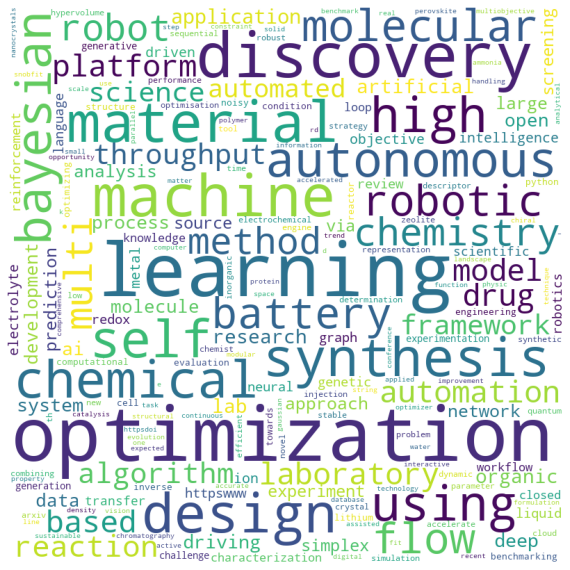
\includegraphics[width=0.5\linewidth]{wordcloud.png}
%     \caption{\small SDL-related key words in \cite{sterling2024}.}
%     \label{fig:wordcloud}
% \end{figure}
This analysis will examine:
\begin{itemize}
    \item Author counts and disciplinary backgrounds
    \item Citation impact and degree of automation related to team structure
    \item Changes in team composition across articles with differing degrees of automation, and over time as automation diffuses
    \end{itemize}
Additionally, curriculum vitae data from SDL authors will help analyze their career mobility and trajectories, assessing labor demand characteristics (e.g., academia versus industry) and the influence of SDL experience on their professional paths, and conducting gender disparity analyses inferred from profile images or names. 

Our analysis builds on established research showing that smaller teams tend to produce more disruptive breakthroughs \cite{wu2019large}, while team size in science has grown due to increasing knowledge specialization \cite{jones2009burden}. We will examine whether these dynamics apply to SDL research teams, where the integration of AI and automation may affect ideal team composition. Prior studies indicate that moderately interdisciplinary teams achieve higher citation impact \cite{yegros2015does} and that generalists versus specialists have different advantages depending on the pace of technological change \cite{teodoridis2019creativity}. We will investigate how these patterns manifest in the SDL domain, where both specialist knowledge and interdisciplinary collaboration are essential.

We will also exploit quasi-experimental variation in the relative costs of automation linked to pandemic-related laboratory access and staffing limitations to provide causal estimates of the impact of  team composition on SDL effectiveness.
% Example of efficient figure inclusion
\begin{figure}[H]
    \centering
    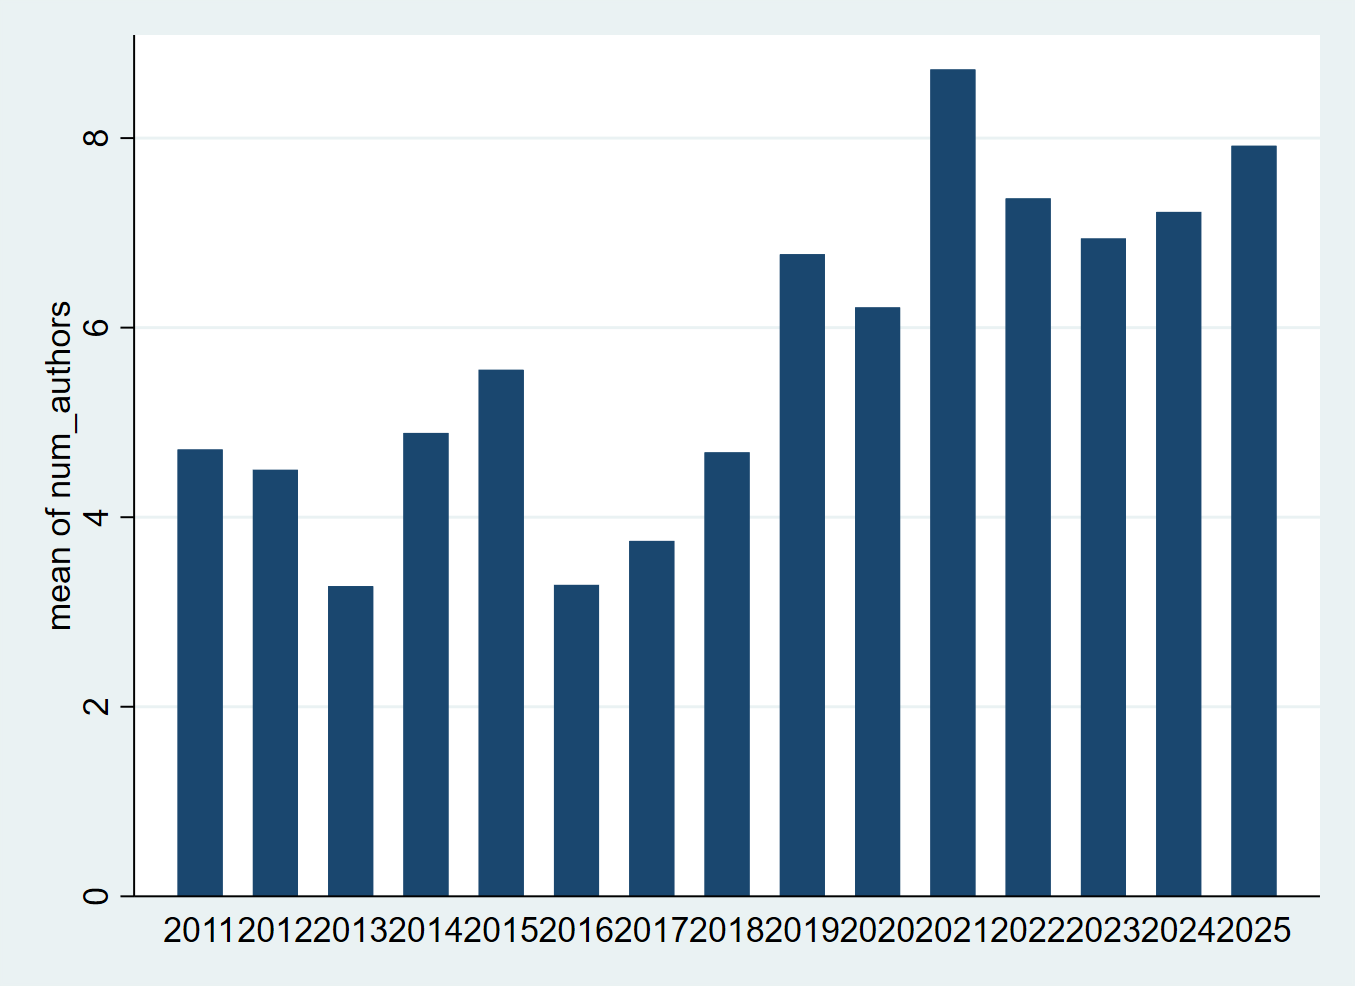
\includegraphics[width=0.9\linewidth]{num_authors.png}
    \caption{\small Average team size in SDL publications over time, demonstrating the evolving collaborative structure in this field. Publications identified using SDL-related key words listed in \cite{sterling2024}.}
    \label{fig:team_size}
\end{figure}

\subsection{Experimental Study}
Building on bibliometric insights, we will conduct a series of hackathon-style experiments in triplicates using chocolate 3D printing as a model SDL system, leveraging chocolate's phase-transition properties as an analog to metals, glass, and plastics:

\begin{itemize}
    \item Teams with varying compositions (e.g., different ratios of MSE, CS, and Mechanical Engineering students) will design autonomous chocolate formulation systems
    \item Specific team compositions will be determined based on our bibliometric findings
    \item Hardware will include chocolate 3D printers, dispensers, and robotic arms, with a \$300 budget per team for additional equipment
    \item Teams will be assessed on degree of automation, product quality, and system flexibility
\end{itemize}

Teams will implement a closed-loop calibration workflow (\cref{fig:chocolate_schematic}):
\begin{enumerate}
    \item Execute a print with a specific chocolate formulation
    \item Transfer the sample to a turntable and capture 360° images
    \item Process images through a provided 3D point cloud reconstruction script to generate digital models \cite{ganitano_hybrid_2024}
    \item Calculate dimensional accuracy by comparing reconstructed and target models \cite{ganitano_hybrid_2024}
    \item Use an optimization algorithm to suggest parameters for the next print
\end{enumerate}

\begin{figure}[t]
    \centering
    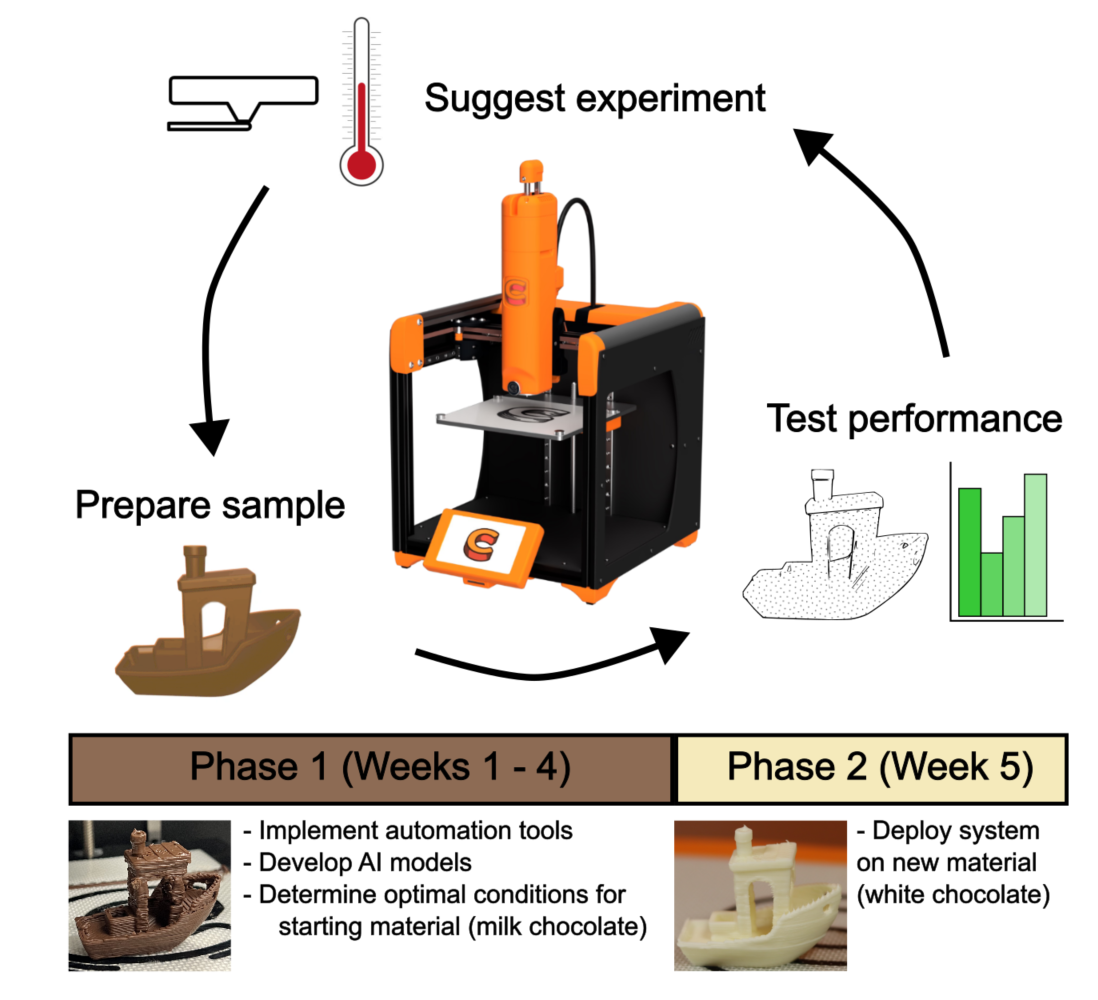
\includegraphics[width=0.45\textwidth]{chocolate-optimization-schematic.png}
    \caption{\small Schematic of our chocolate optimization process, showing how teams interact with the platform. Teams will first optimize milk chocolate parameters, then deploy their system on white chocolate, simulating real-world scenarios.}
    \label{fig:chocolate_schematic}
\end{figure}

\section{Timeline and Deliverables}
\begin{description}[leftmargin=!,labelwidth=\widthof{\bfseries 09/26-04/27:}]
    \item[May-Sep '25:] Data collection, experiment design, pilot studies
    \item[] Implementation of fully autonomous chocolate 3D printing platform, initial hackathon-style experiments
    \item[Sep-Nov '25:] Complete bibliometric analysis, finalize experimental protocols
    \item[Dec '25-May '26:] Run experimental studies, collect and analyze data
    \item[Jun-Aug '26:] Complete integrated analysis of both research components
    \item[Sept '26-Apr '27:] Prepare publications and practitioner guidelines
\end{description}

\section{Budget Summary}
Our budget of \$100,000 is allocated across three main categories:

\begin{itemize}
    \item \textbf{Personnel (\$52,349):} Three full-time undergraduate research assistants for summer bibliometric data collection (\$34,595), plus one part-time research assistant continuing through the academic year (\$16,108)
    
    \item \textbf{Equipment \& Materials (\$31,651):} Three sets of hardware including chocolate 3D printers and robotic arms (\$24,000), chocolate printing materials, sensors, documentation equipment, software licenses, and team budgets (\$7,651)
    
    \item \textbf{Dissemination (\$16,000):} Conference travel for team members (\$15,000) and production of best practices guide (\$1,000)
\end{itemize}

\section{Broader Impact}
This project will directly contribute to the Acceleration Consortium's mission by providing evidence-based strategies for structuring teams that maximize the potential of SDLs, ultimately accelerating materials discovery through optimal human-machine collaboration.

By analyzing team composition, dynamics, and outcomes in a controlled yet relevant setting, our research will offer actionable guidance for assembling effective SDL teams across academia, industry, and government. Our findings will inform best practices that can help scale the impact of SDLs and lower barriers to entry for new institutions seeking to establish their own automated materials discovery programs.

\section{Community Engagement \& EDI Considerations}
Our research design explicitly incorporates equity, diversity, and inclusion (EDI) principles in multiple dimensions:

\begin{itemize}
    \item \textbf{Inclusive Research Team:} Our team reflects a commitment to inclusivity, spanning gender and racial divides, with leadership from early-career and established researchers
    
    \item \textbf{Recruitment Practices:} RA recruitment will prioritize underrepresented backgrounds in STEM; hackathon-style experiments will emphasize diversity across gender, race, and discipline
    
    \item \textbf{Skills Development:} RAs will build both technical and collaborative research skills in a supportive, inclusive environment with intentional rotation of facilitation roles in team meetings to ensure equitable participation
    
    \item \textbf{Inclusive Technology Design:} Our experimental protocols will examine how team diversity affects the accessibility and inclusivity of resulting SDL systems
\end{itemize}

By embedding inclusion throughout the project, we aim to model how diversity strengthens scientific discovery while training the next generation of researchers.

\section{Ethical \& Sustainability Considerations}
We have carefully considered the ethical implications and sustainability of our research:

\begin{itemize}
    \item \textbf{Ethical Data Collection:} All bibliometric analysis and participant studies will follow IRB-approved protocols with proper consent and data anonymization
    \item \textbf{Environmental Sustainability:} Our chocolate-based experimental platform minimizes environmental impact by using biodegradable materials and energy-efficient processes
    \item \textbf{Long-term Impact:} By optimizing team structures for SDLs, we aim to accelerate sustainable materials discovery that addresses pressing global challenges
\end{itemize}

% Can include references as a list here rather than in-line to save space.
\printbibliography

\end{document}